\documentclass[10pt,a4paper]{book}
\usepackage[utf8]{inputenc}							% Codificación
\usepackage[spanish,es-tabla]{babel}				% Lenguaje español, Tabla n: 
\usepackage[T1]{fontenc}							% Agregar fuentes con acentos
\usepackage{amsmath}								% Paquetes necesarios  para matemáticas
\usepackage{amsfonts}
\usepackage{amssymb}
\usepackage{makeidx}								% Paquete para indices
\usepackage{graphicx}								% Para manejar imagenes
\graphicspath{{imagenes/}}							% Ruta de las imagenes, solo escribir nombre de la imagen
\author{Autor}										% Información basica del documento
\title{Titulo}
\date{22 de Julio de 2019 a las 01:03 a.m.}
\addtolength{\marginparsep}{12pt}
\addtolength{\textwidth}{-5pt}


%---------------------------------------------------------------------------------------------------
%-------------------------------------Paquetes adicionales-----------------------------------------
\usepackage[hidelinks]{hyperref}					% Añade los bookmarks y le quita la caja roja, \url{}
\urlstyle{same}
\usepackage{bookmark}									% \url{} con letra normal
\usepackage{bm}

\usepackage{lipsum}									% Rellenar con texto prueba \lipsum[1-20]
\usepackage{calc}									% Hacer calculo numericos
\usepackage{tcolorbox}								% Cuadro de color para resaltar \begin{tcolorbox}...\end{tcolorbox}
\usepackage{comment}								% Comentarios largos \begin{commment}..\end{comment}

\usepackage[hypcap=false]{caption}					% Para agregar figuras en las notas de margen
\captionsetup{										% Configuracion figuras notas de margen
   justification=raggedright
  ,labelfont={bf}
% ,font=footnotesize
}

%---------------------------------------------------------------------------------------------------
%-------------------------------------Encabezados del libro-----------------------------------------
\usepackage{fancyhdr}								% Para cambiar el header y el footer
\pagestyle{fancy}

\fancypagestyle{plain}{								% Quitar numeracion y estilo inicio de capitulo
  \fancyhf{}
}

\renewcommand{\chaptermark}[1]{\markboth{\chaptername\ \thechapter.\ #1}{}}			% Capitulos y secciones en minusculas
\renewcommand{\sectionmark}[1]{\markright{\thesection.\ #1}}

\fancyhf{}											% Reinicial estilos de header y footer
\fancyhead[LE]{\footnotesize\textbf{\thepage}\hspace{\marginparwidth}\hspace{\marginparsep}\textsl{\leftmark}} % Numero de pagina en Izq/par y capitulo
\fancyhead[RO]{\footnotesize\textsl{\rightmark}\hspace{\marginparwidth}\hspace{\marginparsep}\textbf{\thepage}} % Numero de pagina en Der/impar y seccion

\fancyheadoffset[LE,RO]{\marginparsep+\marginparwidth}	% Desplazar header										
\renewcommand{\headrulewidth}{0pt}						% Quitar lineas horizontales en header y footer
\renewcommand{\footrulewidth}{0pt}
%---------------------------------------------------------------------------------------------------
%-------------------------Funciones definidas por el usuario y extras-------------------------------
\decimalpoint										% Punto decimal en lugar de coma
\spanishsignitems									% Viñetas en lugar de cuadros
\raggedbottom

%-------------------------------------------------------
%------Funciones definidas por el usuario y extras------
\usepackage{amsthm}
\newtheorem{thm}{Teorema}[chapter]
\newtheorem{defi}{Definición}[chapter]
\newtheorem{reg}{Regla}[chapter]

\theoremstyle{definition}
\newtheorem{examp}{Ejemplo}[chapter]
										% Arregla algunos warnings

\includeonly{
%				0-portada,
%				1-prefacio,
%				2-notas_al_estudiante,
%				3-acerca_de_los_autores,
				ch1_conceptos_basicos
%				ch2_leyes_basicas,
%				ch3_metodos_de_analisis,
%				Ap-A_ecuaciones_simultaneas_e_inversion_de_matrices,
%				Ap-B_numeros_complejos
			}


\begin{document}
\frontmatter
	
		\begin{titlepage}
		\begin{center}
	        \vspace*{1cm}
	 
	        \Huge
	        \textbf{Thesis Title}
	 
	        \vspace{0.5cm}
	        \LARGE
	        Thesis Subtitle
	 
	        \vspace{1.5cm}
	 
	        \textbf{Author Name}
	 
	        \vfill
	 
	        A thesis presented for the degree of\\
	        Doctor of Philosophy
	 
	        \vspace{0.8cm}
	 
	        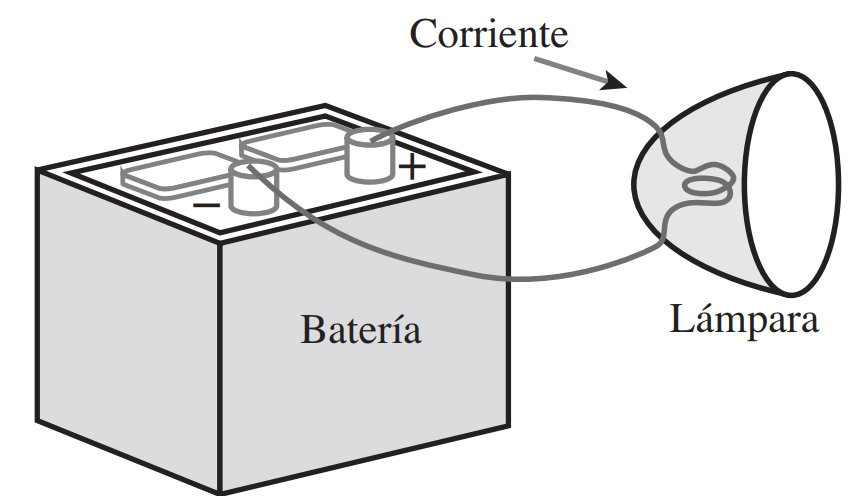
\includegraphics[width=0.4\textwidth]{img1.png}
	 
	        \Large
	        Department Name\\
	        University Name\\
	        Country\\
	        Date
	 
	    \end{center}
	\end{titlepage}

%
%\tableofcontents									% Indice
%\addcontentsline{toc}{chapter}{\contentsname}

\mainmatter

\part{Matemáticas elementales}

	\chapter{Matemáticas elementales}
		
			
		\section{Introducción}
		
		El sistema de los números reales de que ahora disponemos, es el resultado de una enorme cantidad de reflexión por parte del hombre. Los enteros positivos, es decir, $1, 2, 3, \ldots $ , pueden encontrarse desde el comienzo de nuestra civilización. Enteros tan grandes como 100 000 se usaban en Egipto en una fecha tan temprana como es 3 000 antes de cristo. 
		
		Fueron los babilónicos los que más éxito tuvieron en el desarrollo de la aritmética y el álgebra porque tenían una notación para los números muy superior a la de los egipcios. Esta notación era, en principio, análoga a nuestro sistema decimal, excepto por el hecho de que su base era 60 en lugar de 10.
		
		Nuestro sistema decimal con los numerales llamados arábigos fue inventado por los hindúes e introducido a la Europa occidental en el siglo doce a través de las traducciones de textos árabes. Sin embargo la aceptación generalizada de esta notación tardó mucho en llegar.
		
		La aritmética y el álgebra se desarrollaron bajo el estimulo de problemas prácticos y fueron, por ello, comprendimos reglas de ``cómo operar''. En contradicción, la geometría la desarrollaron los griegos solamente para la satisfacción intelectual y es un modelo de sistema lógico.
		
		Disponemos ahora de un sistema de axiomas que describe completamente los números reales; partiendo de estos axiomas podemos derivar todas las propiedades de los números reales. \cite{haaser}
		
		\section{Conjuntos}
		
		Por un ``conjunto'' entendemos  una colección de objetos. Los objetos individuales se llaman ``elementos'' del conjunto.
		
		Si un conjunto tiene un número finito de elementos, entonces se llama conjunto finito; en caso contrario se llama conjunto infinito. El conjunto de enteros desde 1 hasta 10 es un conjunto finito; tiene diez elementos. Un ejemplo de conjunto infinito lo tenemos en el conjunto de todos los enteros positivos.
		
		Se denotan usualmente a los conjuntos con letras manuscritas (mayúsculas) y a sus elementos con letras cursivas minúsculas. Denotaremos el hecho que $b$ sea un elemento del conjunto $\mathcal{B}$ por $b\in \mathcal{B}$. La expresión `` $b \in \mathcal{B}$ '' se lee `` $b$ es un elemento de $\mathcal{B}$ '', `` $b$ pertenece a $\mathcal{B}$ '', o `` $b$ está en $\mathcal{B}$ ''. Un conjunto $\mathcal{B}$ se dice que está definido si, para cualquier elemento $c$, puede determinarse si $c \in \mathcal{B}$ o $c \not\in \mathcal{B}$ (léase `` $c$ no es un elemento de $\mathcal{B}$ '').
		
		Un conjunto finito puede ser mostrado escribiendo sus elementos entre llaves, como: $\{a, b, c\}$. Algunas veces podemos mostrar un conjunto infinito de forma análoga, como en el caso de los enteros positivos: $\{1, 2, 3, \cdots \}$. Los tres puntos quieren decir \textit{etcétera}. Esta notación puede usarse solamente cuando esta claro lo que la palabra etcétera denota. Usualmente, un conjunto infinito se describirá por alguna propiedad que posee cada uno de sus elementos y que no posee objeto alguno que no esté en el conjunto.
		
\vspace{0.21cm}
\begin{tcolorbox}
	\begin{defi}\textbf{Subconjunto}\end{defi}
	Un conjunto $\mathcal{A}$ es un subconjunto de un conjunto $\mathcal{B}$, lo que se denota por $\mathcal{A} \subset \mathcal{B}$, si todo elemento de $\mathcal{A}$ es también elemento de $\mathcal{B}$. $\mathcal{A} \subset \mathcal{B}$ se lee a menudo `` $\mathcal{A}$ está contenido en $\mathcal{B}$ ''.
\end{tcolorbox}

\vspace{0.21cm}
\begin{tcolorbox}
	\begin{defi}\textbf{Intersección}\end{defi}
	La intersección de $\mathcal{A}$ y $\mathcal{B}$, escrita $\mathcal{A} \cap \mathcal{B}$, es el conjunto de elementos que están en ambos $\mathcal{A}$ y $\mathcal{B}$. Es decir, $x \in \mathcal{A} \cap \mathcal{B}$ si y sólo si $x\in \mathcal{A}$ y $x\in \mathcal{B}$.
\end{tcolorbox}

\vspace{0.21cm}
\begin{tcolorbox}
	\begin{defi}\textbf{Unión}\end{defi}
	La unión de $\mathcal{A}$ y $\mathcal{B}$, escrita $\mathcal{A} \cup \mathcal{B}$, es el conjunto de elementos que están en ambos $\mathcal{A}$ o $\mathcal{B}$. Es decir, $x \in \mathcal{A} \cup \mathcal{B}$ si y sólo si $x\in \mathcal{A}$ o $x\in \mathcal{B}$. \footnote{La letra ``o'' tal como se usa en matemáticas tiene el significado ``y/o'' en el lenguaje familiar. Así, `` $x\in \mathcal{A}$ o $x\in \mathcal{B}$ '' significa que $x$ está en $\mathcal{A}$ o en $\mathcal{B}$, o en ambos $\mathcal{A}$ y $\mathcal{B}$.}
\end{tcolorbox}
	
	Para que la intersección de dos conjuntos siempre sea un conjunto, definimos el llamado \textbf{conjunto nulo} o conjunto vacío. Es éste un conjunto sin ningún elemento y se denotará por $\varnothing$.
	
	\vspace{0.21cm}
\begin{tcolorbox}
	\begin{defi}\textbf{Conjunto de números  naturales}\end{defi}
	El conjunto de números naturales se denota por $\mathbb{N}$ y se define como:
		  \[ \mathbb{N} = \{ 1, 2, 3, 4, 5, 6, 7, 8, 9, \ldots \} \]
\end{tcolorbox}

	Entre las propiedades más importantes de los números naturales podemos mencionar la existencia de un orden, la existencia del 1 como primer elemento, que todo número natural tiene otro como sucesor y que todo número natural, excepto el número 1, tiene otro numero natural como antecesor. En términos formales se tiene:
	
	\vspace{1cm}
	\textbf{Propiedades de los números naturales}
	\begin{enumerate}
		\item $1 < n$ para todo $n\in \mathbb{N}$.
		\item Si $k\in \mathbb{N}$ se define su sucesor como $k+1$ y además $k+1 \in \mathbb{N}$.
		\item Si $k\in \mathbb{N}$, $k\neq1$ se define su antecesor como $k-1$ y además $k-1 \in \mathbb{N}$.
	\end{enumerate}
	
	En $\mathbb{N}$ se definen dos operaciones: la suma y el producto. Se verifica que ambas operaciones son cerradas, conmutativas y asociativas, la suma distribuye respecto al producto. El número natural 1 es el neutro multiplicativo, sin embargo, estas propiedades no son suficientes para describir algunos fenómenos físicos, por ejemplo, temperaturas bajo cero, las altitudes por debajo del nivel del mar; en concreto carecen de un elemento neutro aditivo y de inversos aditivos. 	
	
	\vspace{0.21cm}
\marginpar{
	\begin{minipage}[t]{\marginparwidth}
%		\begin{scriptsize}
		\begin{footnotesize}
		$\triangleleft$ Los números naturales están contenidos en los números enteros $\mathbb{N} \subset \mathbb{Z}$.
		\end{footnotesize}
%		\end{scriptsize}
	\end{minipage}
}
\begin{tcolorbox}
	\begin{defi}\textbf{Conjunto de números enteros}\end{defi}
	Se define el conjunto de los números enteros como:
		  \[ \mathbb{Z} = \{ \ldots, -2, -1, 0, 1, 2,\ldots  \} \]
\end{tcolorbox}
	
	En $\mathbb{Z}$ también están definidas las operaciones de suma y producto que son, de nueva cuenta, cerradas, conmutativas y asociativas, también se verifica la propiedad distributiva de la suma, existe el elemento neutro multiplicativo, pero además se agregan el ``cero'' como elemento neutro aditivo y los ``números negativos'' como inversos aditivos. Estas propiedades permiten la definición de la resta como una operación derivada de sumar un número con el inverso aditivo de otro, es decir $x-y = x + (-y)$.
	
	No obstante a lo anterior, la solución a problemas elementales como repartir una naranja entre dos personas o describir qué parte representa un minuto en una hora, o simplemente dar el resultado exacto de dividir 46 dulces entre 5 niños, no puede resolverse en términos de números naturales ni de números enteros. Se hace necesaria, entonces, la introducción de los números fraccionarios, también conocidos como números racionales que tienen otras propiedades de mayor aplicación.
	
	\vspace{0.21cm}
\begin{tcolorbox}
	\begin{defi}\textbf{Conjunto de números racionales}\end{defi}
	Se define el conjunto de los números racionales como:
		  \[ \mathbb{Q} = \left\{ \frac{a}{b} \biggr| a,b \in \mathbb{Z}, b\neq 0 \right\} \]
\end{tcolorbox}
	
	\marginpar{
	\begin{minipage}[t]{\marginparwidth}
%		\begin{scriptsize}
		\begin{footnotesize}
		$\triangleleft$ Todo número entero puede expresarse como el cociente deél mismo y del 1, de maneraque todo entero es un número racional.
		\end{footnotesize}
%		\end{scriptsize}
	\end{minipage}
}
	Los números racionales históricamente se definen como cocientes de números enteros, la condición es que el denominador sea diferente de cero. Dado que todo número entero $n$ puede expresarse como el cociente  $\frac{n}{1}$, entonces se considera que todo número entero es un número racional. Es decir $\mathbb{N} \subset \mathbb{Z} \subset \mathbb{Q}$.
	
Todas las propiedades de los enteros siguen siendo válidas en $\mathbb{Q}$, pero además se verifica la existencia de los inversos multiplicativos para cualquier número racional, excepto el cero. Si $\frac{a}{b} \in \mathbb{Q}$ el inverso multiplicativo se define por  $\frac{b}{a} \in \mathbb{Q}$ y satisface  $\frac{a}{b} \frac{b}{a} = 1$. Se define la división de dos números como el producto de uno por el inverso de otro distinto de cero, esto es $\frac{a}{b} = a \cdot \frac{1}{b} = a \cdot b^{-1}$.
	
\begin{tcolorbox}[colback=blue!12!white]
	\begin{thm} \end{thm}
	Todo número racional puede expresarse como una expansión decimal finita o como una expansión decimal infinita periódica.
\end{tcolorbox}

\begin{examp}{\textbf{Una expansión decimal finita es un número racional}}

	\noindent Demostrar que la expansión decimal 0.14 es un número racional.
	
	\vspace{0.5cm}
	
	\noindent \textbf{Solución:}
	\begin{eqnarray*}
		\mbox{Si } x = 0.14 \mbox{ entonces} &  & \\
		x = 0.14 &  & \qquad \qquad \leftarrow \mbox{multiplicar por }10^2\\
		100 x = 14 &  & \qquad \qquad \leftarrow \mbox{despejar}\\
		x = \frac{14}{100} = \frac{7}{50}& &
	\end{eqnarray*}
\end{examp}

Dados dos números racionales cualesquiera, siempre es posible determinar un nuevo número racional comprendido entre ellos, esto puede realizarse tantas veces como se desee; por ejemplo, entre los racionales $m$ y $n$ se encuentra el número racional $(m + n)/2$. Sin embargo, los números racionales no ``llenan'' toda la recta numérica.

Al intentar responder preguntas como: ¿cuál es la longitud de la arista de un cuadrado que tiene área 2? o ¿cuál es la razón entre el perímetro de una circunferencia y su radio?, encontramos que las respuestas $\sqrt{2}$ y $\pi$, respectivamente, no pueden expresarse como un número racional. Números de este tipo se conocen como irracionales y gráficamente se “intercalan” en toda la recta numérica en los ``huecos'' que existen entre los elementos del conjunto $\mathbb{Q}$. 

La necesidad de utilizar números irracionales se presentó en algunos problemas de geometría en la Grecia antigua; sin embargo, fue hasta el siglo XIX que se obtuvieron avances significativos gracias a los estudios realizados por Karl Weierstrass, George Cantor y Richard Dedekin.
La construcción total se dio a partir de los axiomas que estableció Giuseppe Peano en 1889.

Los números irracionales son todos aquellos que no pueden expresarse como el cociente de dos enteros, o bien como aquellos números que tienen una expansión decimal \textit{infinita no periódica}. En ocasiones basta entender que los irracionales son un conjunto disjunto de los racionales.

\vspace{0.21cm}
\begin{tcolorbox}
	\begin{defi}\textbf{Conjunto de números irracionales}\end{defi}
	Se define el conjunto de los números irracionales $\mathbb{I}$ como el conjunto de todos los números que no son racionales.
		  \[ \mathbb{I} = \left\{ x | x \mbox{ es una expansión decimal infinita no periódica} \right\} \]
\end{tcolorbox}

\begin{examp}{\textbf{Algunos números irracionales}}

	\noindent Algunos números irracionales son:.
	
	\begin{enumerate}
		\item $e$
		\item $\pi$
		\item $\sqrt{2}$
		\item $\sqrt{p}$, con $p$ número primo.
		\item $a + \sqrt{p}$, si $a$ es un número racional y $p$ un número primo.
	\end{enumerate}
\end{examp}

	\section{Los números reales}
	
	El sistema de los números reales puede definirse suponiendo que se tienen los números racionales y definiendo luego un número real en términos de números racionales. Por otra parte, se puede definir el sistema de números reales por un conjunto de axiomas\footnote{Axioma: es una proposición que se acepta como verdadera sin la necesidad de ser demostrada.} y luego demostrar que los números racionales pueden considerarse como subconjunto de los números reales. Este último es el método que nosotros utilizaremos.
	
	El sistema de los números reales es un conjunto $\mathbb{R}$ sujeto a dos operaciones, adición y multiplicación, junto con una relación de orden, denotada por “$<$” que se lee “menor que”, tal que cumple el axioma del supremo.
	
	Se distinguen tres grupos de axiomas para el conjunto de números reales:
	
\begin{enumerate}
	\item Axiomas de campo (referente a las operaciones adición y multiplicación).
	\item Axiomas de orden (que se refieren a la relación “ser menor que”).
	\item Axioma del supremo (también referente a la relación de orden).
\end{enumerate}	
	
\vspace{0.21cm}
\begin{tcolorbox}
	\begin{defi}\textbf{Conjunto de números reales}\end{defi}
	Se define al conjunto de los números reales como la unión disjunta de números racionales e irracionales. Es decir $\mathbb{R} = \mathbb{Q} \cup \mathbb{I}$.
	
Es importante observar que los racionales y los irracionales son conjuntos disjuntos, esto es, que dado un número real o está en $\mathbb{Q}$ o está en $\mathbb{I}$ pero nunca en ambos. Además se verifican las contenciones propias:

		  \[ \mathbb{N} \subset \mathbb{Z} \subset \mathbb{Q} \subset \mathbb{R} \qquad  \mbox{e} \qquad \mathbb{I} \subset \mathbb{R}  \]
\end{tcolorbox}

Los números reales satisfacen los siguientes axiomas:

\begin{itemize}
	\item[$\bm{\mathrm{A}_{1}}$] Para todo $a$ y $b$ en $\mathbb{R}$, $a+b \in \mathbb{R}$.  \textbf{(Estabilidad o “cerradura”.)}
	\item[$\bm{\mathrm{A}_{2}}$] Para todo $a$ y $b$ en $\mathbb{R}$, $a+b = b+a$. \textbf{(Ley conmutativa.)}
	\item[$\bm{\mathrm{A}_{3}}$] Para todo $a$, $b$ y $c$ en $\mathbb{R}$, $(a+b)+c = a +(b+c)$. \textbf{(Ley asociativa.)}
	\item[$\bm{\mathrm{A}_{4}}$] Hay un elemento y sólo un elemento, al que denotamos por “$0$”, tal que para todo $a$ en $\mathbb{R}$, $a+0 = a = 0+a$. \textbf{(La existencia y unicidad del elemento neutro aditivo.)}
	\item[$\bm{\mathrm{A}_{5}}$] Para cada  $a$ en $\mathbb{R}$, hay un y sólo un elemento, al que denotamos por “$-a$”, tal que $a+(-a) = 0 = -a + a$. \textbf{(La existencia y unicidad del inverso aditivo.)}
	
	\item[$\bm{\mathrm{M}_{1}}$] Para todo $a$ y $b$ en $\mathbb{R}$, $ab \in \mathbb{R}$.  \textbf{(Estabilidad.)}
	\item[$\bm{\mathrm{M}_{2}}$] Para todo $a$ y $b$ en $\mathbb{R}$, $ab = ba$. \textbf{(Ley conmutativa.)}
	\item[$\bm{\mathrm{M}_{3}}$] Para todo $a$, $b$ y $c$ en $\mathbb{R}$, $(ab)c = a(bc)$. \textbf{(Ley asociativa.)}
	\item[$\bm{\mathrm{M}_{4}}$] Hay un elemento y sólo un elemento, al que denotamos por “$1$”, diferente de 0, tal que para todo $a$ en $\mathbb{R}$, $a\cdot 1 = a = 1\cdot a$. \textbf{(La existencia y unicidad del elemento neutro multiplicativo.)}
	\item[$\bm{\mathrm{M}_{5}}$] Para cada  $a$ en $\mathbb{R}$, diferente de $0$, hay un y sólo un elemento, al que denotamos por $a^{-1}$, tal que $a\cdot a^{-1} = 1 = a^{-1} \cdot a$. \textbf{(La existencia y unicidad del inverso multiplicativo.)}
	
	\item[$\bm{\mathrm{D}}$] Para todo $a, b$ y $c$ en $\mathbb{R}$, $a(b+c) = ab + ac$ y  $(b+c)a = ba + ca$ \textbf{(Ley distributiva.)}
	
	\item[$\bm{\mathrm{O}_{1}}$] Para cualesquiera dos elementos $a$ y $b$ en $\mathbb{R}$ una y solamente una de las siguientes relaciones se verifica: $a<b$, $a = b$, $a>b$. \textbf{(Ley de tricotomía.)}
	\item[$\bm{\mathrm{O}_{2}}$] Si $a<b$ y $b<c$, entonces $a<c$. \textbf{(Ley transitiva.)}
	\item[$\bm{\mathrm{O}_{3}}$] Si $a<b$, entonces, para todo $c$ en $\mathbb{R}$,  $a+c < b+c$.
	\item[$\bm{\mathrm{O}_{4}}$] Si $a<b$ y $0<c$, entonces $ac<bc$.
	\item[$\bm{\mathrm{L}}$] El axioma del supremo (se estudiará a profundidad posteriormente). 
	\marginpar{
	\begin{minipage}[t]{\marginparwidth}
%		\begin{scriptsize}
		\begin{footnotesize}
		$\triangleright$ Este axioma es el que distingue el sistema de los números reales del sistema de los números racionales. El sistema de los números racionales satisface todos los axiomas del sistema de los números reales, excepto el axioma del supremo.
		\end{footnotesize}
%		\end{scriptsize}
	\end{minipage}
}
\end{itemize}


	Todas las propiedades conocidas de los números reales pueden demostrarse a partir de los axiomas anteriores, por esta razón se dice que la teoría de los números reales es una \textit{teoría axiomática}.
	
	Si todos los axiomas  $\bm{\mathrm{A}_{n}}$, $\bm{\mathrm{M}_{n}}$ y $\bm{\mathrm{D}}$, se cumplieran en algún conjunto, este conjunto se llamaría \textbf{campo}. Un campo que cumpla con todos los axiomas $\bm{\mathrm{O}_{n}}$ se llamará \textbf{campo ordenado}. A un campo ordenado que cumpla $\bm{\mathrm{L}}$, se le llamará \textbf{campo ordenado completo}. Por todo lo anterior los números reales son un campo ordenado completo.
	
	\vspace{0.21cm}
\begin{tcolorbox}[colback=blue!12!white]
	\begin{thm} Otras propuiedades de orden\end{thm}
	\begin{enumerate}
		\item Si $0 < y$ y $0 <x$, entonces $0 <xy$.
		\item Si $y < x$ y $z <0$, entonces $yz > xz$.
		\item Si $0<x$ y $0<y$, entonces $0 < x+y$.
		
		\item Si $0<y<x$ y $0<w<z$, entonces $y+w < x+z$.
		\item Si $0<y<x$ y $0<w<z$, entonces $yw < xz$.
	\end{enumerate}
\end{tcolorbox}

\newpage
Para poder entender el axioma del supremo primero es necesario conocer las siguientes definiciones:


\vspace{0.21cm}

\marginpar{
	\begin{minipage}[t]{\marginparwidth}
%		\begin{scriptsize}
		\begin{footnotesize}
		$\triangleleft$ Se presentan dos definiciones totalmente equivalentes para mayor comprensión. 
		\end{footnotesize}
%		\end{scriptsize}
	\end{minipage}
}
\begin{tcolorbox}
	\begin{defi}\textbf{Cota superior}\end{defi}
	Un conjunto $\mathcal{S}$ de números reales está \textbf{acotado superiormente} (o tiene una cota superior) si existe un número $c$ tal qué, para todo $x \in \mathcal{S}$, $x \leq c$. Un cualquier tal número $c$ se lama \textbf{cota superior} de $\mathcal{S}$. \cite{haaser}
	
\vspace{0.5cm}
Sea $\mathcal{A} \subset \mathbb{R}$, si existe $x \in \mathbb{R}$ tal que  $a \leq x$ para todo $a \in \mathcal{A}$, entonces $x$ se llama una cota superior de $\mathcal{A}$ y se dice que el conjunto $\mathcal{A}$ está acotado por arriba o que $\mathcal{A}$ está acotado superiormente. \cite{zill}
\end{tcolorbox}

\vspace{0.21cm}
\begin{tcolorbox}
	\begin{defi}\textbf{Cota inferior}\end{defi}
	Un conjunto $\mathcal{S}$ de números reales está \textbf{acotado inferiormente} (o tiene una cota inferior) si existe un número $c$ tal qué, para todo $x \in \mathcal{S}$, $x \geq c$. Un cualquier tal número $c$ se lama \textbf{cota inferior} de $\mathcal{S}$.
	
\vspace{0.5cm}
Sea $\mathcal{A} \subset \mathbb{R}$, si existe $x \in \mathbb{R}$ tal que  $x \leq a$ para todo $a \in \mathcal{A}$, entonces $x$ se llama una cota inferior de $\mathcal{A}$ y se dice que el conjunto $\mathcal{A}$ está acotado por abajo o que $\mathcal{A}$ está acotado inferiormente. \cite{zill}
\end{tcolorbox}

\vspace{0.21cm}
\begin{tcolorbox}
	\begin{defi}\textbf{Acotado}\end{defi}
	Un conjunto $\mathcal{S}$ de números reales está \textbf{acotado}  si existe un número $c$ tal qué para todo $x \in \mathcal{S}$, $|x| \leq c$.
	
	Es fácil ver que un conjunto $\mathcal{S}$ está acotado sy y sólo si es superiormente e inferiormente acotado, ya que $|x| \leq c$ es equivalente a $-c \leq x \leq c$.
\end{tcolorbox}

\vspace{0.21cm}
\begin{tcolorbox}
	\begin{defi}\textbf{Supremo}\end{defi}
	Un número $c$ se llama \textbf{supremo} de un conjunto $\mathcal{S}$, lo que escribimos $c = \mathrm{sup}\, \mathcal{S}$, si $c$ es una cota superior de $\mathcal{S}$ y ningún número menor que $c$ es una cota superior de $\mathcal{S}$.
	
	Como cualquier número menor que $c$ puede escribirse como $c-\varepsilon$  donde $\varepsilon > 0$, podemos reformular la anterior definición de la siguiente manera:
	
	\vspace{0.35cm}
	$c = \mathrm{sup} \,\mathcal{S}$ si:
	
	\begin{enumerate}
		\item para todo $x \in \mathcal{S}$, $x \leq c$, y
		\item para cualquier $\varepsilon > 0$ existe un $x \in \mathcal{S}$ tal que $x > c - \varepsilon$. \cite{haaser}
	\end{enumerate}
	
	
	Sea $\mathcal{A} \subset \mathbb{R}$ un conjunto acotado por arriba y supongamos que existe $x\in \mathbb{R}$ que satisface las siguientes dos condiciones:
	
	\begin{itemize}
		\item $x$ es una cota superior de $\mathcal{A}$.
		\item Si $y$ es una cota superior de $\mathcal{A}$, entonces $x \leq y$.
	\end{itemize}
	Entonces $x$ se dice el supremo de $\mathcal{A}$ y tiene la propiedad de ser “la menor de todas las cotas superiores”. \cite{zill}
\end{tcolorbox}
		



\vspace{0.21cm}
\begin{tcolorbox}
	\begin{defi}\textbf{Infimo}\end{defi}
	Un número $c$ se llama \textbf{ínfimo} de un conjunto $\mathcal{S}$, lo que escribimos $c = \text{ínf} \, \mathcal{S}$, si $c$ es una cota inferior de $\mathcal{S}$ y ningún número mayor que $c$ es una cota inferior de $\mathcal{S}$.
	
	Como cualquier número mayor que $c$ puede escribirse como $c+\varepsilon$  donde $\varepsilon > 0$, podemos reformular la anterior definición de la siguiente manera:
	
	\vspace{0.35cm}
	$c = \text{ínf} \,\mathcal{S}$ si:
	
	\begin{enumerate}
		\item para todo $x \in \mathcal{S}$, $c \leq x$, y
		\item para cualquier $\varepsilon > 0$ existe un $x \in \mathcal{S}$ tal que $x < c + \varepsilon$. \cite{haaser}
	\end{enumerate}
	
	
	Sea $\mathcal{A} \subset \mathbb{R}$ un conjunto acotado por abajo y supongamos que existe $x\in \mathbb{R}$ que satisface las siguientes dos condiciones:
	
	\begin{itemize}
		\item $x$ es una cota inferior de $\mathcal{A}$.
		\item Si $y$ es una cota inferior de $\mathcal{A}$, entonces $y \leq x$.
	\end{itemize}
	Entonces $x$ se dice el ínfimo de $\mathcal{A}$ y tiene la propiedad de ser “la mayor de todas las cotas inferiores”. \cite{zill}
\end{tcolorbox}



\appendix
	


\backmatter

\begin{thebibliography}{99}
	\bibitem{haaser} Haaser, N., La Salle, J. y Sullivan, J. Análisis Matemático I. Vol. 1 y 2. Ed. Trillas. 1978.
	\bibitem{zill} Zill, Dennis G. Matemáticas 1 Cálculo diferencial  4a. ed. McGraw-Hill/Interamericana. México, 2011.
\end{thebibliography}

\end{document}